\documentclass[1p]{elsarticle_modified}
%\bibliographystyle{elsarticle-num}

%\usepackage[colorlinks]{hyperref}
%\usepackage{abbrmath_seonhwa} %\Abb, \Ascr, \Acal ,\Abf, \Afrak
\usepackage{amsfonts}
\usepackage{amssymb}
\usepackage{amsmath}
\usepackage{amsthm}
\usepackage{scalefnt}
\usepackage{amsbsy}
\usepackage{kotex}
\usepackage{caption}
\usepackage{subfig}
\usepackage{color}
\usepackage{graphicx}
\usepackage{xcolor} %% white, black, red, green, blue, cyan, magenta, yellow
\usepackage{float}
\usepackage{setspace}
\usepackage{hyperref}

\usepackage{tikz}
\usetikzlibrary{arrows}

\usepackage{multirow}
\usepackage{array} % fixed length table
\usepackage{hhline}

%%%%%%%%%%%%%%%%%%%%%
\makeatletter
\renewcommand*\env@matrix[1][\arraystretch]{%
	\edef\arraystretch{#1}%
	\hskip -\arraycolsep
	\let\@ifnextchar\new@ifnextchar
	\array{*\c@MaxMatrixCols c}}
\makeatother %https://tex.stackexchange.com/questions/14071/how-can-i-increase-the-line-spacing-in-a-matrix
%%%%%%%%%%%%%%%

\usepackage[normalem]{ulem}

\newcommand{\msout}[1]{\ifmmode\text{\sout{\ensuremath{#1}}}\else\sout{#1}\fi}
%SOURCE: \msout is \stkout macro in https://tex.stackexchange.com/questions/20609/strikeout-in-math-mode

\newcommand{\cancel}[1]{
	\ifmmode
	{\color{red}\msout{#1}}
	\else
	{\color{red}\sout{#1}}
	\fi
}

\newcommand{\add}[1]{
	{\color{blue}\uwave{#1}}
}

\newcommand{\replace}[2]{
	\ifmmode
	{\color{red}\msout{#1}}{\color{blue}\uwave{#2}}
	\else
	{\color{red}\sout{#1}}{\color{blue}\uwave{#2}}
	\fi
}

\newcommand{\Sol}{\mathcal{S}} %segment
\newcommand{\D}{D} %diagram
\newcommand{\A}{\mathcal{A}} %arc


%%%%%%%%%%%%%%%%%%%%%%%%%%%%%5 test

\def\sl{\operatorname{\textup{SL}}(2,\Cbb)}
\def\psl{\operatorname{\textup{PSL}}(2,\Cbb)}
\def\quan{\mkern 1mu \triangleright \mkern 1mu}

\theoremstyle{definition}
\newtheorem{thm}{Theorem}[section]
\newtheorem{prop}[thm]{Proposition}
\newtheorem{lem}[thm]{Lemma}
\newtheorem{ques}[thm]{Question}
\newtheorem{cor}[thm]{Corollary}
\newtheorem{defn}[thm]{Definition}
\newtheorem{exam}[thm]{Example}
\newtheorem{rmk}[thm]{Remark}
\newtheorem{alg}[thm]{Algorithm}

\newcommand{\I}{\sqrt{-1}}
\begin{document}

%\begin{frontmatter}
%
%\title{Boundary parabolic representations of knots up to 8 crossings}
%
%%% Group authors per affiliation:
%\author{Yunhi Cho} 
%\address{Department of Mathematics, University of Seoul, Seoul, Korea}
%\ead{yhcho@uos.ac.kr}
%
%
%\author{Seonhwa Kim} %\fnref{s_kim}}
%\address{Center for Geometry and Physics, Institute for Basic Science, Pohang, 37673, Korea}
%\ead{ryeona17@ibs.re.kr}
%
%\author{Hyuk Kim}
%\address{Department of Mathematical Sciences, Seoul National University, Seoul 08826, Korea}
%\ead{hyukkim@snu.ac.kr}
%
%\author{Seokbeom Yoon}
%\address{Department of Mathematical Sciences, Seoul National University, Seoul, 08826,  Korea}
%\ead{sbyoon15@snu.ac.kr}
%
%\begin{abstract}
%We find all boundary parabolic representation of knots up to 8 crossings.
%
%\end{abstract}
%\begin{keyword}
%    \MSC[2010] 57M25 
%\end{keyword}
%
%\end{frontmatter}

%\linenumbers
%\tableofcontents
%
\newcommand\colored[1]{\textcolor{white}{\rule[-0.35ex]{0.8em}{1.4ex}}\kern-0.8em\color{red} #1}%
%\newcommand\colored[1]{\textcolor{white}{ #1}\kern-2.17ex	\textcolor{white}{ #1}\kern-1.81ex	\textcolor{white}{ #1}\kern-2.15ex\color{red}#1	}

{\Large $\underline{12a_{0207}~(K12a_{0207})}$}

\setlength{\tabcolsep}{10pt}
\renewcommand{\arraystretch}{1.6}
\vspace{1cm}\begin{tabular}{m{100pt}>{\centering\arraybackslash}m{274pt}}
\multirow{5}{120pt}{
	\centering
	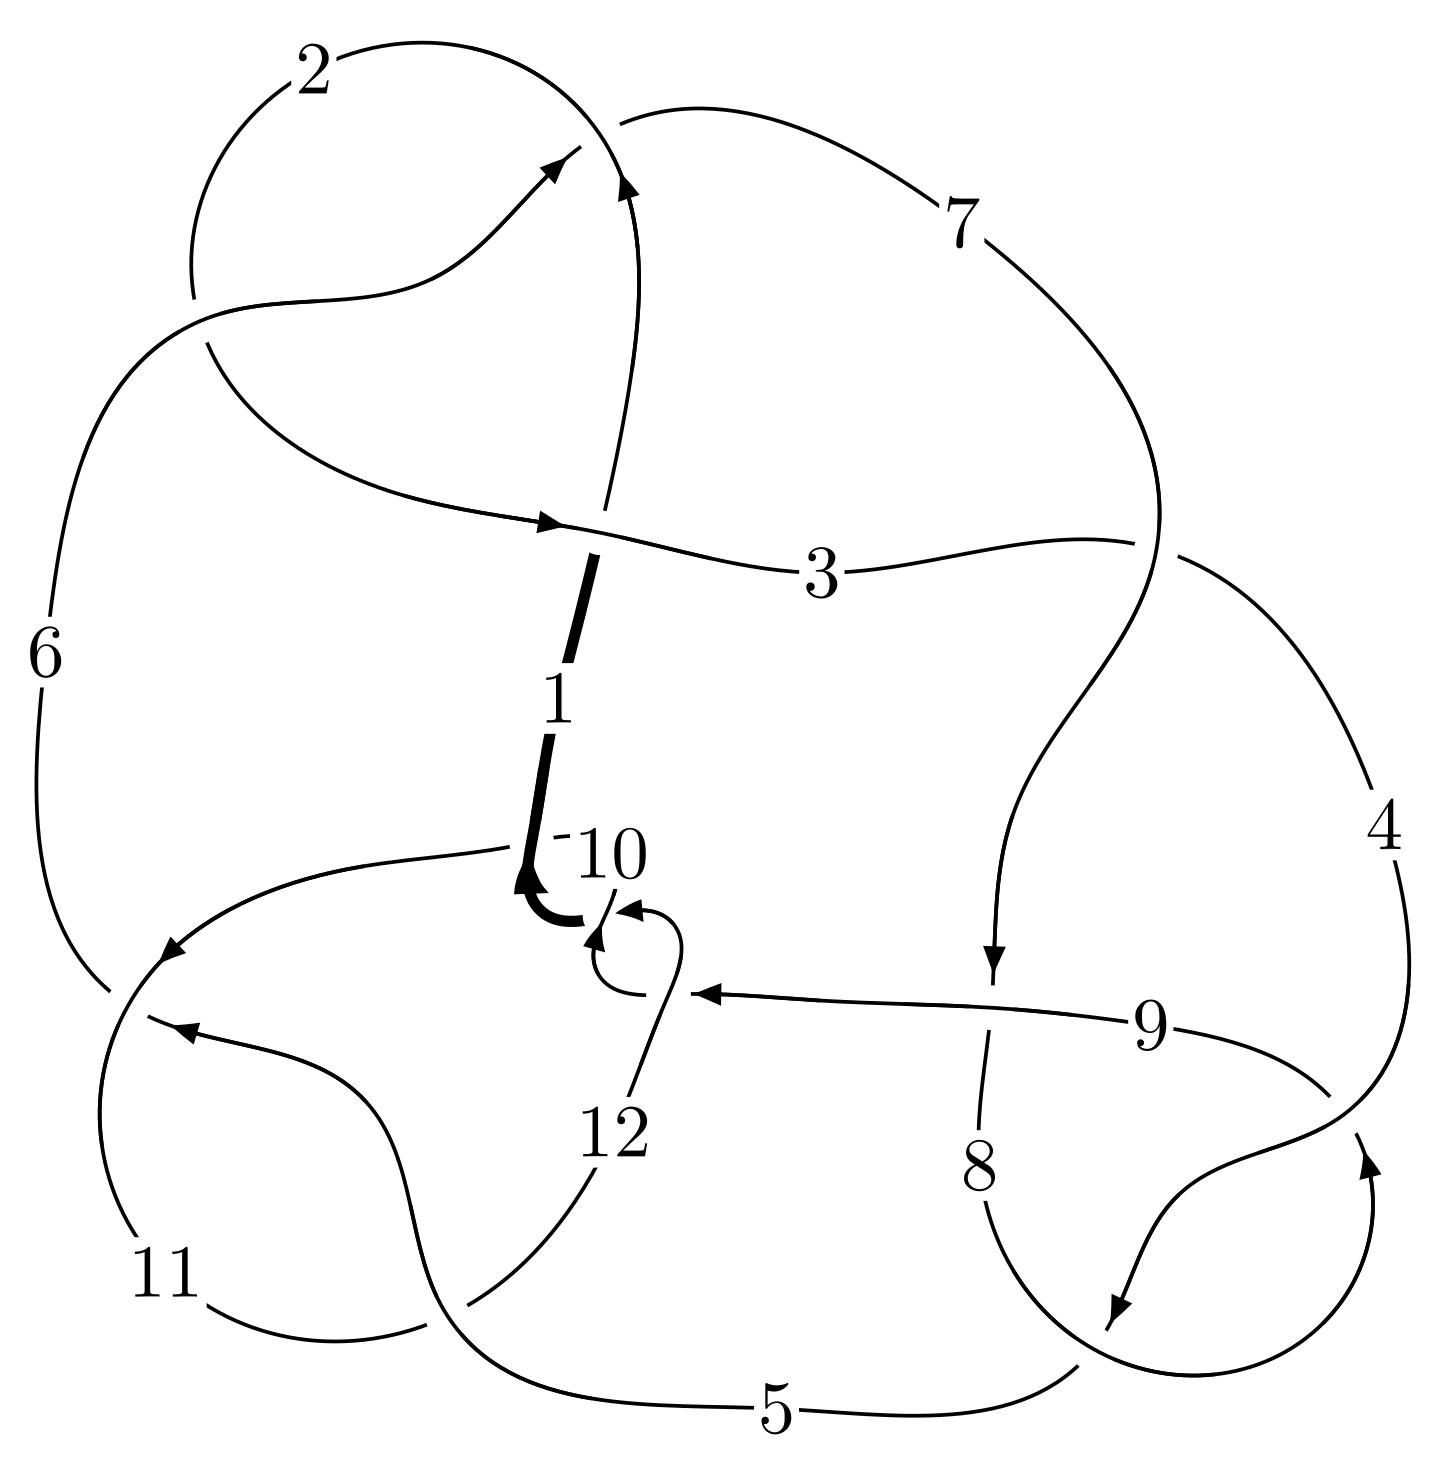
\includegraphics[width=112pt]{../../../GIT/diagram.site/Diagrams/png/1008_12a_0207.png}\\
\ \ \ A knot diagram\footnotemark}&
\allowdisplaybreaks
\textbf{Linearized knot diagam} \\
\cline{2-2}
 &
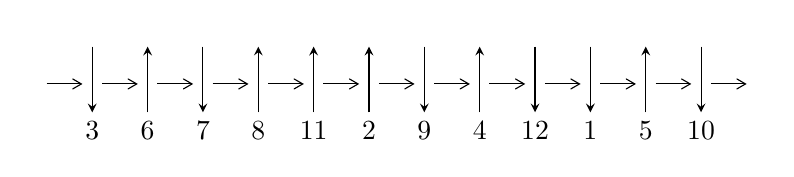
\begin{tikzpicture}[x=20pt, y=17pt]
	% nodes
	\node (C0) at (0, 0) {};
	\node (C1) at (1, 0) {};
	\node (C1U) at (1, +1) {};
	\node (C1D) at (1, -1) {3};

	\node (C2) at (2, 0) {};
	\node (C2U) at (2, +1) {};
	\node (C2D) at (2, -1) {6};

	\node (C3) at (3, 0) {};
	\node (C3U) at (3, +1) {};
	\node (C3D) at (3, -1) {7};

	\node (C4) at (4, 0) {};
	\node (C4U) at (4, +1) {};
	\node (C4D) at (4, -1) {8};

	\node (C5) at (5, 0) {};
	\node (C5U) at (5, +1) {};
	\node (C5D) at (5, -1) {11};

	\node (C6) at (6, 0) {};
	\node (C6U) at (6, +1) {};
	\node (C6D) at (6, -1) {2};

	\node (C7) at (7, 0) {};
	\node (C7U) at (7, +1) {};
	\node (C7D) at (7, -1) {9};

	\node (C8) at (8, 0) {};
	\node (C8U) at (8, +1) {};
	\node (C8D) at (8, -1) {4};

	\node (C9) at (9, 0) {};
	\node (C9U) at (9, +1) {};
	\node (C9D) at (9, -1) {12};

	\node (C10) at (10, 0) {};
	\node (C10U) at (10, +1) {};
	\node (C10D) at (10, -1) {1};

	\node (C11) at (11, 0) {};
	\node (C11U) at (11, +1) {};
	\node (C11D) at (11, -1) {5};

	\node (C12) at (12, 0) {};
	\node (C12U) at (12, +1) {};
	\node (C12D) at (12, -1) {10};
	\node (C13) at (13, 0) {};

	% arrows
	\draw[->,>={angle 60}]
	(C0) edge (C1) (C1) edge (C2) (C2) edge (C3) (C3) edge (C4) (C4) edge (C5) (C5) edge (C6) (C6) edge (C7) (C7) edge (C8) (C8) edge (C9) (C9) edge (C10) (C10) edge (C11) (C11) edge (C12) (C12) edge (C13) ;	\draw[->,>=stealth]
	(C1U) edge (C1D) (C2D) edge (C2U) (C3U) edge (C3D) (C4D) edge (C4U) (C5D) edge (C5U) (C6D) edge (C6U) (C7U) edge (C7D) (C8D) edge (C8U) (C9U) edge (C9D) (C10U) edge (C10D) (C11D) edge (C11U) (C12U) edge (C12D) ;
	\end{tikzpicture} \\
\hhline{~~} \\& 
\textbf{Solving Sequence} \\ \cline{2-2} 
 &
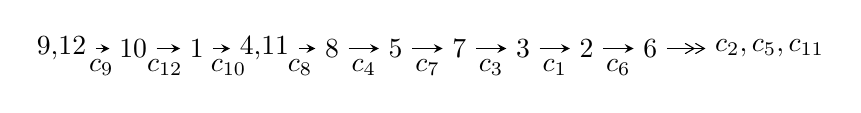
\begin{tikzpicture}[x=23pt, y=7pt]
	% node
	\node (A0) at (-1/8, 0) {9,12};
	\node (A1) at (1, 0) {10};
	\node (A2) at (2, 0) {1};
	\node (A3) at (49/16, 0) {4,11};
	\node (A4) at (33/8, 0) {8};
	\node (A5) at (41/8, 0) {5};
	\node (A6) at (49/8, 0) {7};
	\node (A7) at (57/8, 0) {3};
	\node (A8) at (65/8, 0) {2};
	\node (A9) at (73/8, 0) {6};
	\node (C1) at (1/2, -1) {$c_{9}$};
	\node (C2) at (3/2, -1) {$c_{12}$};
	\node (C3) at (5/2, -1) {$c_{10}$};
	\node (C4) at (29/8, -1) {$c_{8}$};
	\node (C5) at (37/8, -1) {$c_{4}$};
	\node (C6) at (45/8, -1) {$c_{7}$};
	\node (C7) at (53/8, -1) {$c_{3}$};
	\node (C8) at (61/8, -1) {$c_{1}$};
	\node (C9) at (69/8, -1) {$c_{6}$};
	\node (A10) at (11, 0) {$c_{2},c_{5},c_{11}$};

	% edge
	\draw[->,>=stealth]	
	(A0) edge (A1) (A1) edge (A2) (A2) edge (A3) (A3) edge (A4) (A4) edge (A5) (A5) edge (A6) (A6) edge (A7) (A7) edge (A8) (A8) edge (A9) ;
	\draw[->>,>={angle 60}]	
	(A9) edge (A10);
\end{tikzpicture} \\ 

\end{tabular} \\

\footnotetext{
The image of knot diagram is generated by the software ``\textbf{Draw programme}" developed by Andrew Bartholomew(\url{http://www.layer8.co.uk/maths/draw/index.htm\#Running-draw}), where we modified some parts for our purpose(\url{https://github.com/CATsTAILs/LinksPainter}).
}\phantom \\ \newline 
\centering \textbf{Ideals for irreducible components\footnotemark of $X_{\text{par}}$} 
 
\begin{align*}
I^u_{1}&=\langle 
-1.51570\times10^{15} u^{34}-5.53502\times10^{15} u^{33}+\cdots+1.20230\times10^{15} b+4.04644\times10^{15},\\
\phantom{I^u_{1}}&\phantom{= \langle  }6.68182\times10^{15} u^{34}+2.49675\times10^{16} u^{33}+\cdots+4.80919\times10^{15} a-2.62648\times10^{16},\;u^{35}+5 u^{34}+\cdots-13 u-4\rangle \\
I^u_{2}&=\langle 
-1763 u^{28} a+3881 u^{28}+\cdots-1262 a+2496,\;29 u^{28} a-5 u^{28}+\cdots+5 a+39,\;u^{29}+4 u^{28}+\cdots+2 u+1\rangle \\
I^u_{3}&=\langle 
-2 a^2+b+a+1,\;2 a^4- a^3-2 a^2+a+1,\;u-1\rangle \\
I^u_{4}&=\langle 
a^5- a^4-3 a^3+4 a^2+b+4 a-2,\;a^6-2 a^5- a^4+5 a^3-3 a+1,\;u-1\rangle \\
I^u_{5}&=\langle 
a u+b+u+1,\;a^2+2 a u+4 a+4 u+7,\;u^2+u-1\rangle \\
\\
\end{align*}
\raggedright * 5 irreducible components of $\dim_{\mathbb{C}}=0$, with total 107 representations.\\
\footnotetext{All coefficients of polynomials are rational numbers. But the coefficients are sometimes approximated in decimal forms when there is not enough margin.}
\newpage
\renewcommand{\arraystretch}{1}
\centering \section*{I. $I^u_{1}= \langle -1.52\times10^{15} u^{34}-5.54\times10^{15} u^{33}+\cdots+1.20\times10^{15} b+4.05\times10^{15},\;6.68\times10^{15} u^{34}+2.50\times10^{16} u^{33}+\cdots+4.81\times10^{15} a-2.63\times10^{16},\;u^{35}+5 u^{34}+\cdots-13 u-4 \rangle$}
\flushleft \textbf{(i) Arc colorings}\\
\begin{tabular}{m{7pt} m{180pt} m{7pt} m{180pt} }
\flushright $a_{9}=$&$\begin{pmatrix}1\\0\end{pmatrix}$ \\
\flushright $a_{12}=$&$\begin{pmatrix}0\\u\end{pmatrix}$ \\
\flushright $a_{10}=$&$\begin{pmatrix}1\\u^2\end{pmatrix}$ \\
\flushright $a_{1}=$&$\begin{pmatrix}- u\\- u^3+u\end{pmatrix}$ \\
\flushright $a_{4}=$&$\begin{pmatrix}-1.38939 u^{34}-5.19162 u^{33}+\cdots+16.4019 u+5.46137\\1.26067 u^{34}+4.60371 u^{33}+\cdots-11.0154 u-3.36559\end{pmatrix}$ \\
\flushright $a_{11}=$&$\begin{pmatrix}- u^2+1\\- u^4+2 u^2\end{pmatrix}$ \\
\flushright $a_{8}=$&$\begin{pmatrix}-0.955888 u^{34}-3.63380 u^{33}+\cdots+10.9509 u+4.67994\\1.37755 u^{34}+5.16666 u^{33}+\cdots-11.9980 u-4.33307\end{pmatrix}$ \\
\flushright $a_{5}=$&$\begin{pmatrix}-1.18952 u^{34}-4.52016 u^{33}+\cdots+14.1974 u+5.74534\\1.68537 u^{34}+6.13795 u^{33}+\cdots-14.5486 u-4.33555\end{pmatrix}$ \\
\flushright $a_{7}=$&$\begin{pmatrix}0.421659 u^{34}+1.53286 u^{33}+\cdots-1.04716 u+0.346871\\1.37755 u^{34}+5.16666 u^{33}+\cdots-11.9980 u-4.33307\end{pmatrix}$ \\
\flushright $a_{3}=$&$\begin{pmatrix}0.507830 u^{34}+1.85439 u^{33}+\cdots-1.52833 u-0.397819\\1.41127 u^{34}+5.28521 u^{33}+\cdots-12.6990 u-4.42566\end{pmatrix}$ \\
\flushright $a_{2}=$&$\begin{pmatrix}-0.624564 u^{34}-2.20570 u^{33}+\cdots+1.73779 u+1.68599\\-0.299699 u^{34}-1.03425 u^{33}+\cdots+2.40823 u+0.469963\end{pmatrix}$ \\
\flushright $a_{6}=$&$\begin{pmatrix}0.222426 u^{34}+0.604677 u^{33}+\cdots+3.42434 u+2.44151\\1.45957 u^{34}+5.39478 u^{33}+\cdots-13.5630 u-4.01322\end{pmatrix}$\\&\end{tabular}
\flushleft \textbf{(ii) Obstruction class $= -1$}\\~\\
\flushleft \textbf{(iii) Cusp Shapes $= -\frac{28600273364382339}{9618382602850592} u^{34}-\frac{55866542605177373}{4809191301425296} u^{33}+\cdots+\frac{344438964453645221}{9618382602850592} u+\frac{38144347486615397}{2404595650712648}$}\\~\\
\newpage\renewcommand{\arraystretch}{1}
\flushleft \textbf{(iv) u-Polynomials at the component}\newline \\
\begin{tabular}{m{50pt}|m{274pt}}
Crossings & \hspace{64pt}u-Polynomials at each crossing \\
\hline $$\begin{aligned}c_{1},c_{7}\end{aligned}$$&$\begin{aligned}
&u^{35}+18 u^{34}+\cdots-9 u-1
\end{aligned}$\\
\hline $$\begin{aligned}c_{2},c_{4},c_{6}\\c_{8}\end{aligned}$$&$\begin{aligned}
&u^{35}+9 u^{33}+\cdots- u-1
\end{aligned}$\\
\hline $$\begin{aligned}c_{3}\end{aligned}$$&$\begin{aligned}
&u^{35}+6 u^{34}+\cdots+64 u-64
\end{aligned}$\\
\hline $$\begin{aligned}c_{5},c_{11}\end{aligned}$$&$\begin{aligned}
&u^{35}+3 u^{34}+\cdots-112 u+64
\end{aligned}$\\
\hline $$\begin{aligned}c_{9},c_{10},c_{12}\end{aligned}$$&$\begin{aligned}
&u^{35}-5 u^{34}+\cdots-13 u+4
\end{aligned}$\\
\hline
\end{tabular}\\~\\
\newpage\renewcommand{\arraystretch}{1}
\flushleft \textbf{(v) Riley Polynomials at the component}\newline \\
\begin{tabular}{m{50pt}|m{274pt}}
Crossings & \hspace{64pt}Riley Polynomials at each crossing \\
\hline $$\begin{aligned}c_{1},c_{7}\end{aligned}$$&$\begin{aligned}
&y^{35}+6 y^{34}+\cdots+3 y-1
\end{aligned}$\\
\hline $$\begin{aligned}c_{2},c_{4},c_{6}\\c_{8}\end{aligned}$$&$\begin{aligned}
&y^{35}+18 y^{34}+\cdots-9 y-1
\end{aligned}$\\
\hline $$\begin{aligned}c_{3}\end{aligned}$$&$\begin{aligned}
&y^{35}-24 y^{34}+\cdots-57344 y-4096
\end{aligned}$\\
\hline $$\begin{aligned}c_{5},c_{11}\end{aligned}$$&$\begin{aligned}
&y^{35}+27 y^{34}+\cdots-7936 y-4096
\end{aligned}$\\
\hline $$\begin{aligned}c_{9},c_{10},c_{12}\end{aligned}$$&$\begin{aligned}
&y^{35}-37 y^{34}+\cdots-175 y-16
\end{aligned}$\\
\hline
\end{tabular}\\~\\
\newpage\flushleft \textbf{(vi) Complex Volumes and Cusp Shapes}
$$\begin{array}{c|c|c}  
\text{Solutions to }I^u_{1}& \I (\text{vol} + \sqrt{-1}CS) & \text{Cusp shape}\\
 \hline 
\begin{aligned}
u &= \phantom{-}0.959008 + 0.270609 I \\
a &= \phantom{-}0.823234 + 0.223651 I \\
b &= -0.173746 + 0.485732 I\end{aligned}
 & -1.84314 - 0.87084 I & -4.62038 + 1.34519 I \\ \hline\begin{aligned}
u &= \phantom{-}0.959008 - 0.270609 I \\
a &= \phantom{-}0.823234 - 0.223651 I \\
b &= -0.173746 - 0.485732 I\end{aligned}
 & -1.84314 + 0.87084 I & -4.62038 - 1.34519 I \\ \hline\begin{aligned}
u &= \phantom{-}0.512518 + 0.917994 I \\
a &= -1.70850 + 0.05834 I \\
b &= \phantom{-}0.517624 - 1.215310 I\end{aligned}
 & -7.59221 - 11.92590 I & -6.11495 + 8.82041 I \\ \hline\begin{aligned}
u &= \phantom{-}0.512518 - 0.917994 I \\
a &= -1.70850 - 0.05834 I \\
b &= \phantom{-}0.517624 + 1.215310 I\end{aligned}
 & -7.59221 + 11.92590 I & -6.11495 - 8.82041 I \\ \hline\begin{aligned}
u &= \phantom{-}0.954171 + 0.487790 I \\
a &= \phantom{-}0.010990 + 0.441890 I \\
b &= -0.416864 - 0.843498 I\end{aligned}
 & -2.25613 + 2.35480 I & -4.42628 - 5.78689 I \\ \hline\begin{aligned}
u &= \phantom{-}0.954171 - 0.487790 I \\
a &= \phantom{-}0.010990 - 0.441890 I \\
b &= -0.416864 + 0.843498 I\end{aligned}
 & -2.25613 - 2.35480 I & -4.42628 + 5.78689 I \\ \hline\begin{aligned}
u &= \phantom{-}0.721919 + 0.835340 I \\
a &= -0.372316 - 0.313834 I \\
b &= \phantom{-}0.476440 + 1.196050 I\end{aligned}
 & -8.22119 + 6.06183 I & -7.41980 - 3.98537 I \\ \hline\begin{aligned}
u &= \phantom{-}0.721919 - 0.835340 I \\
a &= -0.372316 + 0.313834 I \\
b &= \phantom{-}0.476440 - 1.196050 I\end{aligned}
 & -8.22119 - 6.06183 I & -7.41980 + 3.98537 I \\ \hline\begin{aligned}
u &= \phantom{-}0.495421 + 0.731154 I \\
a &= \phantom{-}1.122580 + 0.574754 I \\
b &= -0.732884 - 0.119482 I\end{aligned}
 & -1.27974 - 2.37099 I & \phantom{-}0.31894 + 3.15329 I \\ \hline\begin{aligned}
u &= \phantom{-}0.495421 - 0.731154 I \\
a &= \phantom{-}1.122580 - 0.574754 I \\
b &= -0.732884 + 0.119482 I\end{aligned}
 & -1.27974 + 2.37099 I & \phantom{-}0.31894 - 3.15329 I\\
 \hline 
 \end{array}$$\newpage$$\begin{array}{c|c|c}  
\text{Solutions to }I^u_{1}& \I (\text{vol} + \sqrt{-1}CS) & \text{Cusp shape}\\
 \hline 
\begin{aligned}
u &= \phantom{-}0.200040 + 0.713689 I \\
a &= \phantom{-}1.50067 - 1.01116 I \\
b &= -0.551950 + 0.938432 I\end{aligned}
 & \phantom{-}0.02332 - 6.64372 I & -0.26642 + 9.39853 I \\ \hline\begin{aligned}
u &= \phantom{-}0.200040 - 0.713689 I \\
a &= \phantom{-}1.50067 + 1.01116 I \\
b &= -0.551950 - 0.938432 I\end{aligned}
 & \phantom{-}0.02332 + 6.64372 I & -0.26642 - 9.39853 I \\ \hline\begin{aligned}
u &= \phantom{-}1.283430 + 0.258737 I \\
a &= -1.16481 - 0.94463 I \\
b &= \phantom{-}0.468567 - 0.922566 I\end{aligned}
 & -2.99912 - 4.93329 I & -3.82940 + 6.57606 I \\ \hline\begin{aligned}
u &= \phantom{-}1.283430 - 0.258737 I \\
a &= -1.16481 + 0.94463 I \\
b &= \phantom{-}0.468567 + 0.922566 I\end{aligned}
 & -2.99912 + 4.93329 I & -3.82940 - 6.57606 I \\ \hline\begin{aligned}
u &= -1.365140 + 0.043173 I \\
a &= -0.965795 + 0.425482 I \\
b &= \phantom{-}0.760139 - 0.637733 I\end{aligned}
 & -2.59101 - 0.97059 I & -3.20816 + 2.30460 I \\ \hline\begin{aligned}
u &= -1.365140 - 0.043173 I \\
a &= -0.965795 - 0.425482 I \\
b &= \phantom{-}0.760139 + 0.637733 I\end{aligned}
 & -2.59101 + 0.97059 I & -3.20816 - 2.30460 I \\ \hline\begin{aligned}
u &= \phantom{-}1.39159\phantom{ +0.000000I} \\
a &= \phantom{-}0.0610608\phantom{ +0.000000I} \\
b &= \phantom{-}0.727022\phantom{ +0.000000I}\end{aligned}
 & -3.41993\phantom{ +0.000000I} & -0.649850\phantom{ +0.000000I} \\ \hline\begin{aligned}
u &= -1.389770 + 0.195625 I \\
a &= \phantom{-}1.45955 - 0.21134 I \\
b &= -0.651228 - 1.025580 I\end{aligned}
 & -4.98605 + 9.79445 I & -5.34481 - 8.93651 I \\ \hline\begin{aligned}
u &= -1.389770 - 0.195625 I \\
a &= \phantom{-}1.45955 + 0.21134 I \\
b &= -0.651228 + 1.025580 I\end{aligned}
 & -4.98605 - 9.79445 I & -5.34481 + 8.93651 I \\ \hline\begin{aligned}
u &= -0.481446 + 0.181091 I \\
a &= \phantom{-}1.21465 - 1.46620 I \\
b &= -0.528136 - 1.141240 I\end{aligned}
 & -3.37780 + 7.99798 I & \phantom{-}0.71148 - 7.40743 I\\
 \hline 
 \end{array}$$\newpage$$\begin{array}{c|c|c}  
\text{Solutions to }I^u_{1}& \I (\text{vol} + \sqrt{-1}CS) & \text{Cusp shape}\\
 \hline 
\begin{aligned}
u &= -0.481446 - 0.181091 I \\
a &= \phantom{-}1.21465 + 1.46620 I \\
b &= -0.528136 + 1.141240 I\end{aligned}
 & -3.37780 - 7.99798 I & \phantom{-}0.71148 + 7.40743 I \\ \hline\begin{aligned}
u &= \phantom{-}1.51965 + 0.08089 I \\
a &= \phantom{-}0.71051 + 1.32043 I \\
b &= -0.495431 + 1.212500 I\end{aligned}
 & -10.12230 - 9.08658 I & \phantom{-0.000000 } 0 \\ \hline\begin{aligned}
u &= \phantom{-}1.51965 - 0.08089 I \\
a &= \phantom{-}0.71051 - 1.32043 I \\
b &= -0.495431 - 1.212500 I\end{aligned}
 & -10.12230 + 9.08658 I & \phantom{-0.000000 } 0 \\ \hline\begin{aligned}
u &= -0.100508 + 0.458939 I \\
a &= -2.27911 + 0.05270 I \\
b &= \phantom{-}0.543260 + 0.738488 I\end{aligned}
 & \phantom{-}1.32849 + 2.20779 I & \phantom{-}4.23160 - 4.03649 I \\ \hline\begin{aligned}
u &= -0.100508 - 0.458939 I \\
a &= -2.27911 - 0.05270 I \\
b &= \phantom{-}0.543260 - 0.738488 I\end{aligned}
 & \phantom{-}1.32849 - 2.20779 I & \phantom{-}4.23160 + 4.03649 I \\ \hline\begin{aligned}
u &= -1.52211 + 0.26355 I \\
a &= \phantom{-}0.493088 - 0.569107 I \\
b &= -0.872759 + 0.176459 I\end{aligned}
 & -7.85990 + 6.04546 I & \phantom{-0.000000 } 0 \\ \hline\begin{aligned}
u &= -1.52211 - 0.26355 I \\
a &= \phantom{-}0.493088 + 0.569107 I \\
b &= -0.872759 - 0.176459 I\end{aligned}
 & -7.85990 - 6.04546 I & \phantom{-0.000000 } 0 \\ \hline\begin{aligned}
u &= -1.55878 + 0.33189 I \\
a &= -1.50039 + 0.85083 I \\
b &= \phantom{-}0.543971 + 1.243490 I\end{aligned}
 & -14.3234 + 16.5120 I & \phantom{-0.000000 } 0 \\ \hline\begin{aligned}
u &= -1.55878 - 0.33189 I \\
a &= -1.50039 - 0.85083 I \\
b &= \phantom{-}0.543971 - 1.243490 I\end{aligned}
 & -14.3234 - 16.5120 I & \phantom{-0.000000 } 0 \\ \hline\begin{aligned}
u &= -1.63807 + 0.22494 I \\
a &= -0.012996 - 0.570463 I \\
b &= \phantom{-}0.408913 - 1.203980 I\end{aligned}
 & -16.1932 - 2.1173 I & \phantom{-0.000000 } 0\\
 \hline 
 \end{array}$$\newpage$$\begin{array}{c|c|c}  
\text{Solutions to }I^u_{1}& \I (\text{vol} + \sqrt{-1}CS) & \text{Cusp shape}\\
 \hline 
\begin{aligned}
u &= -1.63807 - 0.22494 I \\
a &= -0.012996 + 0.570463 I \\
b &= \phantom{-}0.408913 + 1.203980 I\end{aligned}
 & -16.1932 + 2.1173 I & \phantom{-0.000000 } 0 \\ \hline\begin{aligned}
u &= -0.120066 + 0.311369 I \\
a &= \phantom{-}0.23634 + 1.50251 I \\
b &= \phantom{-}0.516750 - 0.437851 I\end{aligned}
 & \phantom{-}1.051550 - 0.797647 I & \phantom{-}6.50655 + 3.66562 I \\ \hline\begin{aligned}
u &= -0.120066 - 0.311369 I \\
a &= \phantom{-}0.23634 - 1.50251 I \\
b &= \phantom{-}0.516750 + 0.437851 I\end{aligned}
 & \phantom{-}1.051550 + 0.797647 I & \phantom{-}6.50655 - 3.66562 I \\ \hline\begin{aligned}
u &= -1.66607 + 0.03814 I \\
a &= \phantom{-}0.026783 + 0.627545 I \\
b &= -0.176178 + 0.879030 I\end{aligned}
 & -11.63190 - 0.88202 I & \phantom{-0.000000 } 0 \\ \hline\begin{aligned}
u &= -1.66607 - 0.03814 I \\
a &= \phantom{-}0.026783 - 0.627545 I \\
b &= -0.176178 - 0.879030 I\end{aligned}
 & -11.63190 + 0.88202 I & \phantom{-0.000000 } 0\\
 \hline 
 \end{array}$$\newpage\newpage\renewcommand{\arraystretch}{1}
\centering \section*{II. $I^u_{2}= \langle -1763 u^{28} a+3881 u^{28}+\cdots-1262 a+2496,\;29 u^{28} a-5 u^{28}+\cdots+5 a+39,\;u^{29}+4 u^{28}+\cdots+2 u+1 \rangle$}
\flushleft \textbf{(i) Arc colorings}\\
\begin{tabular}{m{7pt} m{180pt} m{7pt} m{180pt} }
\flushright $a_{9}=$&$\begin{pmatrix}1\\0\end{pmatrix}$ \\
\flushright $a_{12}=$&$\begin{pmatrix}0\\u\end{pmatrix}$ \\
\flushright $a_{10}=$&$\begin{pmatrix}1\\u^2\end{pmatrix}$ \\
\flushright $a_{1}=$&$\begin{pmatrix}- u\\- u^3+u\end{pmatrix}$ \\
\flushright $a_{4}=$&$\begin{pmatrix}a\\1.52773 a u^{28}-3.36308 u^{28}+\cdots+1.09359 a-2.16291\end{pmatrix}$ \\
\flushright $a_{11}=$&$\begin{pmatrix}- u^2+1\\- u^4+2 u^2\end{pmatrix}$ \\
\flushright $a_{8}=$&$\begin{pmatrix}3.11308 a u^{28}-0.363518 u^{28}+\cdots+1.91291 a-0.0706239\\-1.71274 a u^{28}+2.52773 u^{28}+\cdots-1.18674 a+0.593588\end{pmatrix}$ \\
\flushright $a_{5}=$&$\begin{pmatrix}-\frac{5}{2} u^{28}-\frac{11}{2} u^{27}+\cdots-\frac{11}{2} u-\frac{1}{2}\\\frac{5}{4} u^{28}+\frac{13}{4} u^{27}+\cdots+\frac{1}{4} u+\frac{7}{4}\end{pmatrix}$ \\
\flushright $a_{7}=$&$\begin{pmatrix}1.40035 a u^{28}+2.16421 u^{28}+\cdots+0.726170 a+0.522964\\-1.71274 a u^{28}+2.52773 u^{28}+\cdots-1.18674 a+0.593588\end{pmatrix}$ \\
\flushright $a_{3}=$&$\begin{pmatrix}2.86092 a u^{28}-2.45234 u^{28}+\cdots+2.62435 a-3.15165\\3.70147 a u^{28}-4.98960 u^{28}+\cdots+2.58622 a-3.71490\end{pmatrix}$ \\
\flushright $a_{2}=$&$\begin{pmatrix}-3.90945 a u^{28}+1.96274 u^{28}+\cdots-4.28813 a+2.43674\\-6.43718 a u^{28}+5.32582 u^{28}+\cdots-4.88172 a+3.59965\end{pmatrix}$ \\
\flushright $a_{6}=$&$\begin{pmatrix}\frac{9}{2} u^{28}+\frac{25}{2} u^{27}+\cdots+\frac{1}{2} u+\frac{9}{2}\\\frac{19}{4} u^{28}+\frac{51}{4} u^{27}+\cdots+\frac{11}{4} u+\frac{17}{4}\end{pmatrix}$\\&\end{tabular}
\flushleft \textbf{(ii) Obstruction class $= -1$}\\~\\
\flushleft \textbf{(iii) Cusp Shapes $= 9 u^{28}+\frac{49}{2} u^{27}+\cdots+10 u+\frac{3}{2}$}\\~\\
\newpage\renewcommand{\arraystretch}{1}
\flushleft \textbf{(iv) u-Polynomials at the component}\newline \\
\begin{tabular}{m{50pt}|m{274pt}}
Crossings & \hspace{64pt}u-Polynomials at each crossing \\
\hline $$\begin{aligned}c_{1},c_{7}\end{aligned}$$&$\begin{aligned}
&u^{58}+34 u^{57}+\cdots+432 u+81
\end{aligned}$\\
\hline $$\begin{aligned}c_{2},c_{4},c_{6}\\c_{8}\end{aligned}$$&$\begin{aligned}
&u^{58}-2 u^{57}+\cdots-24 u+9
\end{aligned}$\\
\hline $$\begin{aligned}c_{3}\end{aligned}$$&$\begin{aligned}
&(u^{29}-2 u^{28}+\cdots-15 u+9)^{2}
\end{aligned}$\\
\hline $$\begin{aligned}c_{5},c_{11}\end{aligned}$$&$\begin{aligned}
&(u^{29}- u^{28}+\cdots-4 u+8)^{2}
\end{aligned}$\\
\hline $$\begin{aligned}c_{9},c_{10},c_{12}\end{aligned}$$&$\begin{aligned}
&(u^{29}-4 u^{28}+\cdots+2 u-1)^{2}
\end{aligned}$\\
\hline
\end{tabular}\\~\\
\newpage\renewcommand{\arraystretch}{1}
\flushleft \textbf{(v) Riley Polynomials at the component}\newline \\
\begin{tabular}{m{50pt}|m{274pt}}
Crossings & \hspace{64pt}Riley Polynomials at each crossing \\
\hline $$\begin{aligned}c_{1},c_{7}\end{aligned}$$&$\begin{aligned}
&y^{58}-22 y^{57}+\cdots-31428 y+6561
\end{aligned}$\\
\hline $$\begin{aligned}c_{2},c_{4},c_{6}\\c_{8}\end{aligned}$$&$\begin{aligned}
&y^{58}+34 y^{57}+\cdots+432 y+81
\end{aligned}$\\
\hline $$\begin{aligned}c_{3}\end{aligned}$$&$\begin{aligned}
&(y^{29}-24 y^{28}+\cdots+621 y-81)^{2}
\end{aligned}$\\
\hline $$\begin{aligned}c_{5},c_{11}\end{aligned}$$&$\begin{aligned}
&(y^{29}+21 y^{28}+\cdots+144 y-64)^{2}
\end{aligned}$\\
\hline $$\begin{aligned}c_{9},c_{10},c_{12}\end{aligned}$$&$\begin{aligned}
&(y^{29}-30 y^{28}+\cdots+18 y-1)^{2}
\end{aligned}$\\
\hline
\end{tabular}\\~\\
\newpage\flushleft \textbf{(vi) Complex Volumes and Cusp Shapes}
$$\begin{array}{c|c|c}  
\text{Solutions to }I^u_{2}& \I (\text{vol} + \sqrt{-1}CS) & \text{Cusp shape}\\
 \hline 
\begin{aligned}
u &= \phantom{-}0.574714 + 0.809142 I \\
a &= -0.496285 - 0.329278 I \\
b &= \phantom{-}0.383823 + 1.246440 I\end{aligned}
 & -8.55101 - 2.70743 I & -7.83350 + 3.32702 I \\ \hline\begin{aligned}
u &= \phantom{-}0.574714 + 0.809142 I \\
a &= -2.02764 - 0.04424 I \\
b &= \phantom{-}0.430351 - 1.199840 I\end{aligned}
 & -8.55101 - 2.70743 I & -7.83350 + 3.32702 I \\ \hline\begin{aligned}
u &= \phantom{-}0.574714 - 0.809142 I \\
a &= -0.496285 + 0.329278 I \\
b &= \phantom{-}0.383823 - 1.246440 I\end{aligned}
 & -8.55101 + 2.70743 I & -7.83350 - 3.32702 I \\ \hline\begin{aligned}
u &= \phantom{-}0.574714 - 0.809142 I \\
a &= -2.02764 + 0.04424 I \\
b &= \phantom{-}0.430351 + 1.199840 I\end{aligned}
 & -8.55101 + 2.70743 I & -7.83350 - 3.32702 I \\ \hline\begin{aligned}
u &= \phantom{-}0.673518 + 0.754049 I \\
a &= -1.000040 - 0.560059 I \\
b &= \phantom{-}0.769255 - 0.056261 I\end{aligned}
 & -4.91068 + 1.51334 I & -4.49380 - 0.41799 I \\ \hline\begin{aligned}
u &= \phantom{-}0.673518 + 0.754049 I \\
a &= \phantom{-}0.406818 + 0.385726 I \\
b &= -0.411656 - 1.172770 I\end{aligned}
 & -4.91068 + 1.51334 I & -4.49380 - 0.41799 I \\ \hline\begin{aligned}
u &= \phantom{-}0.673518 - 0.754049 I \\
a &= -1.000040 + 0.560059 I \\
b &= \phantom{-}0.769255 + 0.056261 I\end{aligned}
 & -4.91068 - 1.51334 I & -4.49380 + 0.41799 I \\ \hline\begin{aligned}
u &= \phantom{-}0.673518 - 0.754049 I \\
a &= \phantom{-}0.406818 - 0.385726 I \\
b &= -0.411656 + 1.172770 I\end{aligned}
 & -4.91068 - 1.51334 I & -4.49380 + 0.41799 I \\ \hline\begin{aligned}
u &= \phantom{-}0.496046 + 0.855361 I \\
a &= -1.099850 - 0.481039 I \\
b &= \phantom{-}0.852937 + 0.125205 I\end{aligned}
 & -4.33597 - 6.94187 I & -3.09973 + 6.05967 I \\ \hline\begin{aligned}
u &= \phantom{-}0.496046 + 0.855361 I \\
a &= \phantom{-}1.84336 - 0.14503 I \\
b &= -0.491051 + 1.177580 I\end{aligned}
 & -4.33597 - 6.94187 I & -3.09973 + 6.05967 I\\
 \hline 
 \end{array}$$\newpage$$\begin{array}{c|c|c}  
\text{Solutions to }I^u_{2}& \I (\text{vol} + \sqrt{-1}CS) & \text{Cusp shape}\\
 \hline 
\begin{aligned}
u &= \phantom{-}0.496046 - 0.855361 I \\
a &= -1.099850 + 0.481039 I \\
b &= \phantom{-}0.852937 - 0.125205 I\end{aligned}
 & -4.33597 + 6.94187 I & -3.09973 - 6.05967 I \\ \hline\begin{aligned}
u &= \phantom{-}0.496046 - 0.855361 I \\
a &= \phantom{-}1.84336 + 0.14503 I \\
b &= -0.491051 - 1.177580 I\end{aligned}
 & -4.33597 + 6.94187 I & -3.09973 - 6.05967 I \\ \hline\begin{aligned}
u &= \phantom{-}1.09947\phantom{ +0.000000I} \\
a &= -3.27542 + 2.45605 I \\
b &= \phantom{-}0.138638 + 1.028430 I\end{aligned}
 & -5.36254\phantom{ +0.000000I} & \phantom{-}1.86910\phantom{ +0.000000I} \\ \hline\begin{aligned}
u &= \phantom{-}1.09947\phantom{ +0.000000I} \\
a &= -3.27542 - 2.45605 I \\
b &= \phantom{-}0.138638 - 1.028430 I\end{aligned}
 & -5.36254\phantom{ +0.000000I} & \phantom{-}1.86910\phantom{ +0.000000I} \\ \hline\begin{aligned}
u &= \phantom{-}1.109450 + 0.283231 I \\
a &= \phantom{-}1.260760 + 0.513284 I \\
b &= -0.347220 + 0.737093 I\end{aligned}
 & -1.85262 - 1.10103 I & -2.03106 - 0.28755 I \\ \hline\begin{aligned}
u &= \phantom{-}1.109450 + 0.283231 I \\
a &= \phantom{-}0.187734 - 0.187443 I \\
b &= \phantom{-}0.397780 + 0.487721 I\end{aligned}
 & -1.85262 - 1.10103 I & -2.03106 - 0.28755 I \\ \hline\begin{aligned}
u &= \phantom{-}1.109450 - 0.283231 I \\
a &= \phantom{-}1.260760 - 0.513284 I \\
b &= -0.347220 - 0.737093 I\end{aligned}
 & -1.85262 + 1.10103 I & -2.03106 + 0.28755 I \\ \hline\begin{aligned}
u &= \phantom{-}1.109450 - 0.283231 I \\
a &= \phantom{-}0.187734 + 0.187443 I \\
b &= \phantom{-}0.397780 - 0.487721 I\end{aligned}
 & -1.85262 + 1.10103 I & -2.03106 + 0.28755 I \\ \hline\begin{aligned}
u &= -1.377160 + 0.122752 I \\
a &= \phantom{-}0.775794 - 0.486569 I \\
b &= -0.813747 + 0.500062 I\end{aligned}
 & -3.43590 + 4.37313 I & -3.64888 - 4.01970 I \\ \hline\begin{aligned}
u &= -1.377160 + 0.122752 I \\
a &= -1.396230 - 0.037221 I \\
b &= \phantom{-}0.666978 + 0.923318 I\end{aligned}
 & -3.43590 + 4.37313 I & -3.64888 - 4.01970 I\\
 \hline 
 \end{array}$$\newpage$$\begin{array}{c|c|c}  
\text{Solutions to }I^u_{2}& \I (\text{vol} + \sqrt{-1}CS) & \text{Cusp shape}\\
 \hline 
\begin{aligned}
u &= -1.377160 - 0.122752 I \\
a &= \phantom{-}0.775794 + 0.486569 I \\
b &= -0.813747 - 0.500062 I\end{aligned}
 & -3.43590 - 4.37313 I & -3.64888 + 4.01970 I \\ \hline\begin{aligned}
u &= -1.377160 - 0.122752 I \\
a &= -1.396230 + 0.037221 I \\
b &= \phantom{-}0.666978 - 0.923318 I\end{aligned}
 & -3.43590 - 4.37313 I & -3.64888 + 4.01970 I \\ \hline\begin{aligned}
u &= \phantom{-}0.093803 + 0.571484 I \\
a &= \phantom{-}1.77937 + 0.48269 I \\
b &= -0.596648 - 0.524729 I\end{aligned}
 & \phantom{-}1.17976 - 2.10537 I & \phantom{-}3.42367 + 3.98592 I \\ \hline\begin{aligned}
u &= \phantom{-}0.093803 + 0.571484 I \\
a &= -1.13444 + 1.49748 I \\
b &= \phantom{-}0.521180 - 0.791272 I\end{aligned}
 & \phantom{-}1.17976 - 2.10537 I & \phantom{-}3.42367 + 3.98592 I \\ \hline\begin{aligned}
u &= \phantom{-}0.093803 - 0.571484 I \\
a &= \phantom{-}1.77937 - 0.48269 I \\
b &= -0.596648 + 0.524729 I\end{aligned}
 & \phantom{-}1.17976 + 2.10537 I & \phantom{-}3.42367 - 3.98592 I \\ \hline\begin{aligned}
u &= \phantom{-}0.093803 - 0.571484 I \\
a &= -1.13444 - 1.49748 I \\
b &= \phantom{-}0.521180 + 0.791272 I\end{aligned}
 & \phantom{-}1.17976 + 2.10537 I & \phantom{-}3.42367 - 3.98592 I \\ \hline\begin{aligned}
u &= \phantom{-}1.46649 + 0.06834 I \\
a &= -0.79189 - 1.39162 I \\
b &= \phantom{-}0.454670 - 1.185180 I\end{aligned}
 & -6.77922 - 4.29283 I & -4.53955 + 3.19264 I \\ \hline\begin{aligned}
u &= \phantom{-}1.46649 + 0.06834 I \\
a &= -0.0365899 + 0.0197419 I \\
b &= -0.824448 - 0.084249 I\end{aligned}
 & -6.77922 - 4.29283 I & -4.53955 + 3.19264 I \\ \hline\begin{aligned}
u &= \phantom{-}1.46649 - 0.06834 I \\
a &= -0.79189 + 1.39162 I \\
b &= \phantom{-}0.454670 + 1.185180 I\end{aligned}
 & -6.77922 + 4.29283 I & -4.53955 - 3.19264 I \\ \hline\begin{aligned}
u &= \phantom{-}1.46649 - 0.06834 I \\
a &= -0.0365899 - 0.0197419 I \\
b &= -0.824448 + 0.084249 I\end{aligned}
 & -6.77922 + 4.29283 I & -4.53955 - 3.19264 I\\
 \hline 
 \end{array}$$\newpage$$\begin{array}{c|c|c}  
\text{Solutions to }I^u_{2}& \I (\text{vol} + \sqrt{-1}CS) & \text{Cusp shape}\\
 \hline 
\begin{aligned}
u &= \phantom{-}1.46813\phantom{ +0.000000I} \\
a &= \phantom{-}0.70362 + 1.51889 I \\
b &= -0.412156 + 1.228670 I\end{aligned}
 & -10.7199\phantom{ +0.000000I} & -8.58670\phantom{ +0.000000I} \\ \hline\begin{aligned}
u &= \phantom{-}1.46813\phantom{ +0.000000I} \\
a &= \phantom{-}0.70362 - 1.51889 I \\
b &= -0.412156 - 1.228670 I\end{aligned}
 & -10.7199\phantom{ +0.000000I} & -8.58670\phantom{ +0.000000I} \\ \hline\begin{aligned}
u &= -1.46854 + 0.05369 I \\
a &= -0.000804 + 0.602797 I \\
b &= -0.077278 + 1.297810 I\end{aligned}
 & -9.63904 + 2.02688 I & -7.64196 - 3.46616 I \\ \hline\begin{aligned}
u &= -1.46854 + 0.05369 I \\
a &= \phantom{-}1.66820 + 0.63206 I \\
b &= -0.489594 - 0.791303 I\end{aligned}
 & -9.63904 + 2.02688 I & -7.64196 - 3.46616 I \\ \hline\begin{aligned}
u &= -1.46854 - 0.05369 I \\
a &= -0.000804 - 0.602797 I \\
b &= -0.077278 - 1.297810 I\end{aligned}
 & -9.63904 - 2.02688 I & -7.64196 + 3.46616 I \\ \hline\begin{aligned}
u &= -1.46854 - 0.05369 I \\
a &= \phantom{-}1.66820 - 0.63206 I \\
b &= -0.489594 + 0.791303 I\end{aligned}
 & -9.63904 - 2.02688 I & -7.64196 + 3.46616 I \\ \hline\begin{aligned}
u &= \phantom{-}0.332600 + 0.298296 I \\
a &= \phantom{-}1.17191 + 1.35445 I \\
b &= -0.078563 - 1.142090 I\end{aligned}
 & -3.67943 - 0.93878 I & -2.80996 + 7.32576 I \\ \hline\begin{aligned}
u &= \phantom{-}0.332600 + 0.298296 I \\
a &= \phantom{-}2.88434 - 4.02305 I \\
b &= -0.196086 + 0.856959 I\end{aligned}
 & -3.67943 - 0.93878 I & -2.80996 + 7.32576 I \\ \hline\begin{aligned}
u &= \phantom{-}0.332600 - 0.298296 I \\
a &= \phantom{-}1.17191 - 1.35445 I \\
b &= -0.078563 + 1.142090 I\end{aligned}
 & -3.67943 + 0.93878 I & -2.80996 - 7.32576 I \\ \hline\begin{aligned}
u &= \phantom{-}0.332600 - 0.298296 I \\
a &= \phantom{-}2.88434 + 4.02305 I \\
b &= -0.196086 - 0.856959 I\end{aligned}
 & -3.67943 + 0.93878 I & -2.80996 - 7.32576 I\\
 \hline 
 \end{array}$$\newpage$$\begin{array}{c|c|c}  
\text{Solutions to }I^u_{2}& \I (\text{vol} + \sqrt{-1}CS) & \text{Cusp shape}\\
 \hline 
\begin{aligned}
u &= -1.54068 + 0.30648 I \\
a &= -0.461477 + 0.542815 I \\
b &= \phantom{-}0.930068 - 0.139535 I\end{aligned}
 & -10.9685 + 11.1989 I & -5.19156 - 6.17598 I \\ \hline\begin{aligned}
u &= -1.54068 + 0.30648 I \\
a &= \phantom{-}1.56938 - 0.78799 I \\
b &= -0.541040 - 1.210840 I\end{aligned}
 & -10.9685 + 11.1989 I & -5.19156 - 6.17598 I \\ \hline\begin{aligned}
u &= -1.54068 - 0.30648 I \\
a &= -0.461477 - 0.542815 I \\
b &= \phantom{-}0.930068 + 0.139535 I\end{aligned}
 & -10.9685 - 11.1989 I & -5.19156 + 6.17598 I \\ \hline\begin{aligned}
u &= -1.54068 - 0.30648 I \\
a &= \phantom{-}1.56938 + 0.78799 I \\
b &= -0.541040 + 1.210840 I\end{aligned}
 & -10.9685 - 11.1989 I & -5.19156 + 6.17598 I \\ \hline\begin{aligned}
u &= -1.56175 + 0.26987 I \\
a &= \phantom{-}0.005904 - 0.572450 I \\
b &= \phantom{-}0.376897 - 1.308090 I\end{aligned}
 & -15.5682 + 6.6680 I & -9.30046 - 3.89200 I \\ \hline\begin{aligned}
u &= -1.56175 + 0.26987 I \\
a &= -1.71421 + 0.84034 I \\
b &= \phantom{-}0.496073 + 1.194220 I\end{aligned}
 & -15.5682 + 6.6680 I & -9.30046 - 3.89200 I \\ \hline\begin{aligned}
u &= -1.56175 - 0.26987 I \\
a &= \phantom{-}0.005904 + 0.572450 I \\
b &= \phantom{-}0.376897 + 1.308090 I\end{aligned}
 & -15.5682 - 6.6680 I & -9.30046 + 3.89200 I \\ \hline\begin{aligned}
u &= -1.56175 - 0.26987 I \\
a &= -1.71421 - 0.84034 I \\
b &= \phantom{-}0.496073 - 1.194220 I\end{aligned}
 & -15.5682 - 6.6680 I & -9.30046 + 3.89200 I \\ \hline\begin{aligned}
u &= -0.356186 + 0.206024 I \\
a &= -0.329572 - 0.575621 I \\
b &= -0.730042 + 0.234742 I\end{aligned}
 & -0.75685 + 3.25312 I & \phantom{-}3.53153 - 3.58405 I \\ \hline\begin{aligned}
u &= -0.356186 + 0.206024 I \\
a &= -1.75145 + 1.68560 I \\
b &= \phantom{-}0.474813 + 1.053290 I\end{aligned}
 & -0.75685 + 3.25312 I & \phantom{-}3.53153 - 3.58405 I\\
 \hline 
 \end{array}$$\newpage$$\begin{array}{c|c|c}  
\text{Solutions to }I^u_{2}& \I (\text{vol} + \sqrt{-1}CS) & \text{Cusp shape}\\
 \hline 
\begin{aligned}
u &= -0.356186 - 0.206024 I \\
a &= -0.329572 + 0.575621 I \\
b &= -0.730042 - 0.234742 I\end{aligned}
 & -0.75685 - 3.25312 I & \phantom{-}3.53153 + 3.58405 I \\ \hline\begin{aligned}
u &= -0.356186 - 0.206024 I \\
a &= -1.75145 - 1.68560 I \\
b &= \phantom{-}0.474813 - 1.053290 I\end{aligned}
 & -0.75685 - 3.25312 I & \phantom{-}3.53153 + 3.58405 I \\ \hline\begin{aligned}
u &= -1.57403 + 0.21687 I \\
a &= -0.455066 + 0.636664 I \\
b &= \phantom{-}0.779101 - 0.101681 I\end{aligned}
 & -12.38060 + 1.97634 I & -6.56391 + 0. I\phantom{ +0.000000I} \\ \hline\begin{aligned}
u &= -1.57403 + 0.21687 I \\
a &= \phantom{-}0.002336 + 0.579304 I \\
b &= -0.340208 + 1.254970 I\end{aligned}
 & -12.38060 + 1.97634 I & -6.56391 + 0. I\phantom{ +0.000000I} \\ \hline\begin{aligned}
u &= -1.57403 - 0.21687 I \\
a &= -0.455066 - 0.636664 I \\
b &= \phantom{-}0.779101 + 0.101681 I\end{aligned}
 & -12.38060 - 1.97634 I & -6.56391 + 0. I\phantom{ +0.000000I} \\ \hline\begin{aligned}
u &= -1.57403 - 0.21687 I \\
a &= \phantom{-}0.002336 - 0.579304 I \\
b &= -0.340208 - 1.254970 I\end{aligned}
 & -12.38060 - 1.97634 I & -6.56391 + 0. I\phantom{ +0.000000I} \\ \hline\begin{aligned}
u &= -0.304151\phantom{ +0.000000I} \\
a &= \phantom{-}0.71142 + 2.97196 I \\
b &= -0.322825 + 1.145710 I\end{aligned}
 & -4.79354\phantom{ +0.000000I} & -1.88400\phantom{ +0.000000I} \\ \hline\begin{aligned}
u &= -0.304151\phantom{ +0.000000I} \\
a &= \phantom{-}0.71142 - 2.97196 I \\
b &= -0.322825 - 1.145710 I\end{aligned}
 & -4.79354\phantom{ +0.000000I} & -1.88400\phantom{ +0.000000I}\\
 \hline 
 \end{array}$$\newpage\newpage\renewcommand{\arraystretch}{1}
\centering \section*{III. $I^u_{3}= \langle -2 a^2+b+a+1,\;2 a^4- a^3-2 a^2+a+1,\;u-1 \rangle$}
\flushleft \textbf{(i) Arc colorings}\\
\begin{tabular}{m{7pt} m{180pt} m{7pt} m{180pt} }
\flushright $a_{9}=$&$\begin{pmatrix}1\\0\end{pmatrix}$ \\
\flushright $a_{12}=$&$\begin{pmatrix}0\\1\end{pmatrix}$ \\
\flushright $a_{10}=$&$\begin{pmatrix}1\\1\end{pmatrix}$ \\
\flushright $a_{1}=$&$\begin{pmatrix}-1\\0\end{pmatrix}$ \\
\flushright $a_{4}=$&$\begin{pmatrix}a\\2 a^2- a-1\end{pmatrix}$ \\
\flushright $a_{11}=$&$\begin{pmatrix}0\\1\end{pmatrix}$ \\
\flushright $a_{8}=$&$\begin{pmatrix}2 a^3- a^2- a+1\\-2 a^3+a^2-1\end{pmatrix}$ \\
\flushright $a_{5}=$&$\begin{pmatrix}0\\-2 a^3+3 a^2+a-1\end{pmatrix}$ \\
\flushright $a_{7}=$&$\begin{pmatrix}- a\\-2 a^3+a^2-1\end{pmatrix}$ \\
\flushright $a_{3}=$&$\begin{pmatrix}-2 a^3+a^2+a-1\\-2 a^3+a^2-1\end{pmatrix}$ \\
\flushright $a_{2}=$&$\begin{pmatrix}-2 a^3+a^2+a-1\\-2 a^3- a^2+a+1\end{pmatrix}$ \\
\flushright $a_{6}=$&$\begin{pmatrix}0\\-2 a^3+3 a^2+a-1\end{pmatrix}$\\&\end{tabular}
\flushleft \textbf{(ii) Obstruction class $= 1$}\\~\\
\flushleft \textbf{(iii) Cusp Shapes $= 16 a^3-9 a^2-10 a+3$}\\~\\
\newpage\renewcommand{\arraystretch}{1}
\flushleft \textbf{(iv) u-Polynomials at the component}\newline \\
\begin{tabular}{m{50pt}|m{274pt}}
Crossings & \hspace{64pt}u-Polynomials at each crossing \\
\hline $$\begin{aligned}c_{1},c_{7}\end{aligned}$$&$\begin{aligned}
&u^4-2 u^3+3 u^2- u+1
\end{aligned}$\\
\hline $$\begin{aligned}c_{2},c_{4}\end{aligned}$$&$\begin{aligned}
&u^4+u^2+u+1
\end{aligned}$\\
\hline $$\begin{aligned}c_{3}\end{aligned}$$&$\begin{aligned}
&u^4+3 u^3+4 u^2+3 u+2
\end{aligned}$\\
\hline $$\begin{aligned}c_{5},c_{11}\end{aligned}$$&$\begin{aligned}
&u^4
\end{aligned}$\\
\hline $$\begin{aligned}c_{6},c_{8}\end{aligned}$$&$\begin{aligned}
&u^4+u^2- u+1
\end{aligned}$\\
\hline $$\begin{aligned}c_{9},c_{10}\end{aligned}$$&$\begin{aligned}
&(u-1)^4
\end{aligned}$\\
\hline $$\begin{aligned}c_{12}\end{aligned}$$&$\begin{aligned}
&(u+1)^4
\end{aligned}$\\
\hline
\end{tabular}\\~\\
\newpage\renewcommand{\arraystretch}{1}
\flushleft \textbf{(v) Riley Polynomials at the component}\newline \\
\begin{tabular}{m{50pt}|m{274pt}}
Crossings & \hspace{64pt}Riley Polynomials at each crossing \\
\hline $$\begin{aligned}c_{1},c_{7}\end{aligned}$$&$\begin{aligned}
&y^4+2 y^3+7 y^2+5 y+1
\end{aligned}$\\
\hline $$\begin{aligned}c_{2},c_{4},c_{6}\\c_{8}\end{aligned}$$&$\begin{aligned}
&y^4+2 y^3+3 y^2+y+1
\end{aligned}$\\
\hline $$\begin{aligned}c_{3}\end{aligned}$$&$\begin{aligned}
&y^4- y^3+2 y^2+7 y+4
\end{aligned}$\\
\hline $$\begin{aligned}c_{5},c_{11}\end{aligned}$$&$\begin{aligned}
&y^4
\end{aligned}$\\
\hline $$\begin{aligned}c_{9},c_{10},c_{12}\end{aligned}$$&$\begin{aligned}
&(y-1)^4
\end{aligned}$\\
\hline
\end{tabular}\\~\\
\newpage\flushleft \textbf{(vi) Complex Volumes and Cusp Shapes}
$$\begin{array}{c|c|c}  
\text{Solutions to }I^u_{3}& \I (\text{vol} + \sqrt{-1}CS) & \text{Cusp shape}\\
 \hline 
\begin{aligned}
u &= \phantom{-}1.00000\phantom{ +0.000000I} \\
a &= \phantom{-}0.927958 + 0.413327 I \\
b &= -0.547424 + 1.120870 I\end{aligned}
 & -4.26996 - 7.64338 I & -7.31637 + 4.91712 I \\ \hline\begin{aligned}
u &= \phantom{-}1.00000\phantom{ +0.000000I} \\
a &= \phantom{-}0.927958 - 0.413327 I \\
b &= -0.547424 - 1.120870 I\end{aligned}
 & -4.26996 + 7.64338 I & -7.31637 - 4.91712 I \\ \hline\begin{aligned}
u &= \phantom{-}1.00000\phantom{ +0.000000I} \\
a &= -0.677958 + 0.157780 I \\
b &= \phantom{-}0.547424 - 0.585652 I\end{aligned}
 & -0.66484 - 1.39709 I & \phantom{-}1.69137 + 3.76574 I \\ \hline\begin{aligned}
u &= \phantom{-}1.00000\phantom{ +0.000000I} \\
a &= -0.677958 - 0.157780 I \\
b &= \phantom{-}0.547424 + 0.585652 I\end{aligned}
 & -0.66484 + 1.39709 I & \phantom{-}1.69137 - 3.76574 I\\
 \hline 
 \end{array}$$\newpage\newpage\renewcommand{\arraystretch}{1}
\centering \section*{IV. $I^u_{4}= \langle a^5- a^4-3 a^3+4 a^2+b+4 a-2,\;a^6-2 a^5- a^4+5 a^3-3 a+1,\;u-1 \rangle$}
\flushleft \textbf{(i) Arc colorings}\\
\begin{tabular}{m{7pt} m{180pt} m{7pt} m{180pt} }
\flushright $a_{9}=$&$\begin{pmatrix}1\\0\end{pmatrix}$ \\
\flushright $a_{12}=$&$\begin{pmatrix}0\\1\end{pmatrix}$ \\
\flushright $a_{10}=$&$\begin{pmatrix}1\\1\end{pmatrix}$ \\
\flushright $a_{1}=$&$\begin{pmatrix}-1\\0\end{pmatrix}$ \\
\flushright $a_{4}=$&$\begin{pmatrix}a\\- a^5+a^4+3 a^3-4 a^2-4 a+2\end{pmatrix}$ \\
\flushright $a_{11}=$&$\begin{pmatrix}0\\1\end{pmatrix}$ \\
\flushright $a_{8}=$&$\begin{pmatrix}- a^5+2 a^4+a^3-4 a^2- a+2\\2 a^5-3 a^4-3 a^3+7 a^2+4 a-3\end{pmatrix}$ \\
\flushright $a_{5}=$&$\begin{pmatrix}0\\-3 a^5+4 a^4+6 a^3-12 a^2-7 a+5\end{pmatrix}$ \\
\flushright $a_{7}=$&$\begin{pmatrix}a^5- a^4-2 a^3+3 a^2+3 a-1\\2 a^5-3 a^4-3 a^3+7 a^2+4 a-3\end{pmatrix}$ \\
\flushright $a_{3}=$&$\begin{pmatrix}-4 a^5+6 a^4+7 a^3-16 a^2-8 a+7\\-4 a^5+6 a^4+7 a^3-16 a^2-9 a+7\end{pmatrix}$ \\
\flushright $a_{2}=$&$\begin{pmatrix}-4 a^5+6 a^4+7 a^3-16 a^2-8 a+7\\-6 a^5+9 a^4+11 a^3-25 a^2-13 a+12\end{pmatrix}$ \\
\flushright $a_{6}=$&$\begin{pmatrix}0\\-3 a^5+4 a^4+6 a^3-12 a^2-7 a+5\end{pmatrix}$\\&\end{tabular}
\flushleft \textbf{(ii) Obstruction class $= 1$}\\~\\
\flushleft \textbf{(iii) Cusp Shapes $= 10 a^5-13 a^4-20 a^3+39 a^2+23 a-22$}\\~\\
\newpage\renewcommand{\arraystretch}{1}
\flushleft \textbf{(iv) u-Polynomials at the component}\newline \\
\begin{tabular}{m{50pt}|m{274pt}}
Crossings & \hspace{64pt}u-Polynomials at each crossing \\
\hline $$\begin{aligned}c_{1},c_{7}\end{aligned}$$&$\begin{aligned}
&u^6-3 u^5+4 u^4-2 u^3+1
\end{aligned}$\\
\hline $$\begin{aligned}c_{2},c_{4}\end{aligned}$$&$\begin{aligned}
&u^6- u^5+2 u^4-2 u^3+2 u^2-2 u+1
\end{aligned}$\\
\hline $$\begin{aligned}c_{3}\end{aligned}$$&$\begin{aligned}
&(u^3- u^2+1)^2
\end{aligned}$\\
\hline $$\begin{aligned}c_{5},c_{11}\end{aligned}$$&$\begin{aligned}
&u^6
\end{aligned}$\\
\hline $$\begin{aligned}c_{6},c_{8}\end{aligned}$$&$\begin{aligned}
&u^6+u^5+2 u^4+2 u^3+2 u^2+2 u+1
\end{aligned}$\\
\hline $$\begin{aligned}c_{9},c_{10}\end{aligned}$$&$\begin{aligned}
&(u-1)^6
\end{aligned}$\\
\hline $$\begin{aligned}c_{12}\end{aligned}$$&$\begin{aligned}
&(u+1)^6
\end{aligned}$\\
\hline
\end{tabular}\\~\\
\newpage\renewcommand{\arraystretch}{1}
\flushleft \textbf{(v) Riley Polynomials at the component}\newline \\
\begin{tabular}{m{50pt}|m{274pt}}
Crossings & \hspace{64pt}Riley Polynomials at each crossing \\
\hline $$\begin{aligned}c_{1},c_{7}\end{aligned}$$&$\begin{aligned}
&y^6- y^5+4 y^4-2 y^3+8 y^2+1
\end{aligned}$\\
\hline $$\begin{aligned}c_{2},c_{4},c_{6}\\c_{8}\end{aligned}$$&$\begin{aligned}
&y^6+3 y^5+4 y^4+2 y^3+1
\end{aligned}$\\
\hline $$\begin{aligned}c_{3}\end{aligned}$$&$\begin{aligned}
&(y^3- y^2+2 y-1)^2
\end{aligned}$\\
\hline $$\begin{aligned}c_{5},c_{11}\end{aligned}$$&$\begin{aligned}
&y^6
\end{aligned}$\\
\hline $$\begin{aligned}c_{9},c_{10},c_{12}\end{aligned}$$&$\begin{aligned}
&(y-1)^6
\end{aligned}$\\
\hline
\end{tabular}\\~\\
\newpage\flushleft \textbf{(vi) Complex Volumes and Cusp Shapes}
$$\begin{array}{c|c|c}  
\text{Solutions to }I^u_{4}& \I (\text{vol} + \sqrt{-1}CS) & \text{Cusp shape}\\
 \hline 
\begin{aligned}
u &= \phantom{-}1.00000\phantom{ +0.000000I} \\
a &= -1.060970 + 0.237841 I \\
b &= \phantom{-}0.498832 + 1.001300 I\end{aligned}
 & -1.91067 + 2.82812 I & -2.82789 - 2.41717 I \\ \hline\begin{aligned}
u &= \phantom{-}1.00000\phantom{ +0.000000I} \\
a &= -1.060970 - 0.237841 I \\
b &= \phantom{-}0.498832 - 1.001300 I\end{aligned}
 & -1.91067 - 2.82812 I & -2.82789 + 2.41717 I \\ \hline\begin{aligned}
u &= \phantom{-}1.00000\phantom{ +0.000000I} \\
a &= \phantom{-}0.521167 + 0.055259 I \\
b &= -0.713912 - 0.305839 I\end{aligned}
 & -1.91067 - 2.82812 I & -2.82789 + 2.41717 I \\ \hline\begin{aligned}
u &= \phantom{-}1.00000\phantom{ +0.000000I} \\
a &= \phantom{-}0.521167 - 0.055259 I \\
b &= -0.713912 + 0.305839 I\end{aligned}
 & -1.91067 + 2.82812 I & -2.82789 - 2.41717 I \\ \hline\begin{aligned}
u &= \phantom{-}1.00000\phantom{ +0.000000I} \\
a &= \phantom{-}1.53980 + 0.84179 I \\
b &= -0.284920 + 1.115140 I\end{aligned}
 & -6.04826\phantom{ +0.000000I} & -11.34423 + 0. I\phantom{ +0.000000I} \\ \hline\begin{aligned}
u &= \phantom{-}1.00000\phantom{ +0.000000I} \\
a &= \phantom{-}1.53980 - 0.84179 I \\
b &= -0.284920 - 1.115140 I\end{aligned}
 & -6.04826\phantom{ +0.000000I} & -11.34423 + 0. I\phantom{ +0.000000I}\\
 \hline 
 \end{array}$$\newpage\newpage\renewcommand{\arraystretch}{1}
\centering \section*{V. $I^u_{5}= \langle a u+b+u+1,\;a^2+2 a u+4 a+4 u+7,\;u^2+u-1 \rangle$}
\flushleft \textbf{(i) Arc colorings}\\
\begin{tabular}{m{7pt} m{180pt} m{7pt} m{180pt} }
\flushright $a_{9}=$&$\begin{pmatrix}1\\0\end{pmatrix}$ \\
\flushright $a_{12}=$&$\begin{pmatrix}0\\u\end{pmatrix}$ \\
\flushright $a_{10}=$&$\begin{pmatrix}1\\- u+1\end{pmatrix}$ \\
\flushright $a_{1}=$&$\begin{pmatrix}- u\\- u+1\end{pmatrix}$ \\
\flushright $a_{4}=$&$\begin{pmatrix}a\\- a u- u-1\end{pmatrix}$ \\
\flushright $a_{11}=$&$\begin{pmatrix}u\\u\end{pmatrix}$ \\
\flushright $a_{8}=$&$\begin{pmatrix}a u+a+3 u+5\\-1\end{pmatrix}$ \\
\flushright $a_{5}=$&$\begin{pmatrix}- a u- u-1\\0\end{pmatrix}$ \\
\flushright $a_{7}=$&$\begin{pmatrix}a u+a+3 u+4\\-1\end{pmatrix}$ \\
\flushright $a_{3}=$&$\begin{pmatrix}a\\- a u- u-1\end{pmatrix}$ \\
\flushright $a_{2}=$&$\begin{pmatrix}a- u\\- a u-2 u\end{pmatrix}$ \\
\flushright $a_{6}=$&$\begin{pmatrix}a u- a-1\\2 a u- a+u\end{pmatrix}$\\&\end{tabular}
\flushleft \textbf{(ii) Obstruction class $= 1$}\\~\\
\flushleft \textbf{(iii) Cusp Shapes $= -12$}\\~\\
\newpage\renewcommand{\arraystretch}{1}
\flushleft \textbf{(iv) u-Polynomials at the component}\newline \\
\begin{tabular}{m{50pt}|m{274pt}}
Crossings & \hspace{64pt}u-Polynomials at each crossing \\
\hline $$\begin{aligned}c_{1},c_{7}\end{aligned}$$&$\begin{aligned}
&(u-1)^4
\end{aligned}$\\
\hline $$\begin{aligned}c_{2},c_{4},c_{6}\\c_{8}\end{aligned}$$&$\begin{aligned}
&(u^2+1)^2
\end{aligned}$\\
\hline $$\begin{aligned}c_{3}\end{aligned}$$&$\begin{aligned}
&u^4
\end{aligned}$\\
\hline $$\begin{aligned}c_{5},c_{11}\end{aligned}$$&$\begin{aligned}
&u^4+3 u^2+1
\end{aligned}$\\
\hline $$\begin{aligned}c_{9},c_{10}\end{aligned}$$&$\begin{aligned}
&(u^2+u-1)^2
\end{aligned}$\\
\hline $$\begin{aligned}c_{12}\end{aligned}$$&$\begin{aligned}
&(u^2- u-1)^2
\end{aligned}$\\
\hline
\end{tabular}\\~\\
\newpage\renewcommand{\arraystretch}{1}
\flushleft \textbf{(v) Riley Polynomials at the component}\newline \\
\begin{tabular}{m{50pt}|m{274pt}}
Crossings & \hspace{64pt}Riley Polynomials at each crossing \\
\hline $$\begin{aligned}c_{1},c_{7}\end{aligned}$$&$\begin{aligned}
&(y-1)^4
\end{aligned}$\\
\hline $$\begin{aligned}c_{2},c_{4},c_{6}\\c_{8}\end{aligned}$$&$\begin{aligned}
&(y+1)^4
\end{aligned}$\\
\hline $$\begin{aligned}c_{3}\end{aligned}$$&$\begin{aligned}
&y^4
\end{aligned}$\\
\hline $$\begin{aligned}c_{5},c_{11}\end{aligned}$$&$\begin{aligned}
&(y^2+3 y+1)^2
\end{aligned}$\\
\hline $$\begin{aligned}c_{9},c_{10},c_{12}\end{aligned}$$&$\begin{aligned}
&(y^2-3 y+1)^2
\end{aligned}$\\
\hline
\end{tabular}\\~\\
\newpage\flushleft \textbf{(vi) Complex Volumes and Cusp Shapes}
$$\begin{array}{c|c|c}  
\text{Solutions to }I^u_{5}& \I (\text{vol} + \sqrt{-1}CS) & \text{Cusp shape}\\
 \hline 
\begin{aligned}
u &= \phantom{-}0.618034\phantom{ +0.000000I} \\
a &= -2.61803 + 1.61803 I \\
b &= \phantom{-0.000000 } -1.000000 I\end{aligned}
 & -4.27683\phantom{ +0.000000I} & -12.0000\phantom{ +0.000000I} \\ \hline\begin{aligned}
u &= \phantom{-}0.618034\phantom{ +0.000000I} \\
a &= -2.61803 - 1.61803 I \\
b &= \phantom{-0.000000 -}1.000000 I\end{aligned}
 & -4.27683\phantom{ +0.000000I} & -12.0000\phantom{ +0.000000I} \\ \hline\begin{aligned}
u &= -1.61803\phantom{ +0.000000I} \\
a &= -0.381966 + 0.618034 I \\
b &= \phantom{-0.000000 -}1.000000 I\end{aligned}
 & -12.1725\phantom{ +0.000000I} & -12.0000\phantom{ +0.000000I} \\ \hline\begin{aligned}
u &= -1.61803\phantom{ +0.000000I} \\
a &= -0.381966 - 0.618034 I \\
b &= \phantom{-0.000000 } -1.000000 I\end{aligned}
 & -12.1725\phantom{ +0.000000I} & -12.0000\phantom{ +0.000000I}\\
 \hline 
 \end{array}$$\newpage
\newpage\renewcommand{\arraystretch}{1}
\centering \section*{ VI. u-Polynomials}
\begin{tabular}{m{50pt}|m{274pt}}
Crossings & \hspace{64pt}u-Polynomials at each crossing \\
\hline $$\begin{aligned}c_{1},c_{7}\end{aligned}$$&$\begin{aligned}
&(u-1)^4(u^4-2 u^3+3 u^2- u+1)(u^6-3 u^5+4 u^4-2 u^3+1)\\
&\cdot(u^{35}+18 u^{34}+\cdots-9 u-1)(u^{58}+34 u^{57}+\cdots+432 u+81)
\end{aligned}$\\
\hline $$\begin{aligned}c_{2},c_{4}\end{aligned}$$&$\begin{aligned}
&(u^2+1)^2(u^4+u^2+u+1)(u^6- u^5+2 u^4-2 u^3+2 u^2-2 u+1)\\
&\cdot(u^{35}+9 u^{33}+\cdots- u-1)(u^{58}-2 u^{57}+\cdots-24 u+9)
\end{aligned}$\\
\hline $$\begin{aligned}c_{3}\end{aligned}$$&$\begin{aligned}
&u^4(u^3- u^2+1)^2(u^{4}+3 u^{3}+\cdots+3 u+2)(u^{29}-2 u^{28}+\cdots-15 u+9)^{2}\\
&\cdot(u^{35}+6 u^{34}+\cdots+64 u-64)
\end{aligned}$\\
\hline $$\begin{aligned}c_{5},c_{11}\end{aligned}$$&$\begin{aligned}
&u^{10}(u^4+3 u^2+1)(u^{29}- u^{28}+\cdots-4 u+8)^{2}\\
&\cdot(u^{35}+3 u^{34}+\cdots-112 u+64)
\end{aligned}$\\
\hline $$\begin{aligned}c_{6},c_{8}\end{aligned}$$&$\begin{aligned}
&(u^2+1)^2(u^4+u^2- u+1)(u^6+u^5+2 u^4+2 u^3+2 u^2+2 u+1)\\
&\cdot(u^{35}+9 u^{33}+\cdots- u-1)(u^{58}-2 u^{57}+\cdots-24 u+9)
\end{aligned}$\\
\hline $$\begin{aligned}c_{9},c_{10}\end{aligned}$$&$\begin{aligned}
&((u-1)^{10})(u^2+u-1)^2(u^{29}-4 u^{28}+\cdots+2 u-1)^{2}\\
&\cdot(u^{35}-5 u^{34}+\cdots-13 u+4)
\end{aligned}$\\
\hline $$\begin{aligned}c_{12}\end{aligned}$$&$\begin{aligned}
&((u+1)^{10})(u^2- u-1)^2(u^{29}-4 u^{28}+\cdots+2 u-1)^{2}\\
&\cdot(u^{35}-5 u^{34}+\cdots-13 u+4)
\end{aligned}$\\
\hline
\end{tabular}\newpage\renewcommand{\arraystretch}{1}
\centering \section*{ VII. Riley Polynomials}
\begin{tabular}{m{50pt}|m{274pt}}
Crossings & \hspace{64pt}Riley Polynomials at each crossing \\
\hline $$\begin{aligned}c_{1},c_{7}\end{aligned}$$&$\begin{aligned}
&(y-1)^4(y^4+2 y^3+7 y^2+5 y+1)(y^6- y^5+4 y^4-2 y^3+8 y^2+1)\\
&\cdot(y^{35}+6 y^{34}+\cdots+3 y-1)(y^{58}-22 y^{57}+\cdots-31428 y+6561)
\end{aligned}$\\
\hline $$\begin{aligned}c_{2},c_{4},c_{6}\\c_{8}\end{aligned}$$&$\begin{aligned}
&(y+1)^4(y^4+2 y^3+3 y^2+y+1)(y^6+3 y^5+4 y^4+2 y^3+1)\\
&\cdot(y^{35}+18 y^{34}+\cdots-9 y-1)(y^{58}+34 y^{57}+\cdots+432 y+81)
\end{aligned}$\\
\hline $$\begin{aligned}c_{3}\end{aligned}$$&$\begin{aligned}
&y^4(y^3- y^2+2 y-1)^2(y^4- y^3+2 y^2+7 y+4)\\
&\cdot(y^{29}-24 y^{28}+\cdots+621 y-81)^{2}\\
&\cdot(y^{35}-24 y^{34}+\cdots-57344 y-4096)
\end{aligned}$\\
\hline $$\begin{aligned}c_{5},c_{11}\end{aligned}$$&$\begin{aligned}
&y^{10}(y^2+3 y+1)^2(y^{29}+21 y^{28}+\cdots+144 y-64)^{2}\\
&\cdot(y^{35}+27 y^{34}+\cdots-7936 y-4096)
\end{aligned}$\\
\hline $$\begin{aligned}c_{9},c_{10},c_{12}\end{aligned}$$&$\begin{aligned}
&((y-1)^{10})(y^2-3 y+1)^2(y^{29}-30 y^{28}+\cdots+18 y-1)^{2}\\
&\cdot(y^{35}-37 y^{34}+\cdots-175 y-16)
\end{aligned}$\\
\hline
\end{tabular}
\vskip 2pc
\end{document}